\documentclass[cn,10pt,math=newtx,citestyle=gb7714-2015,bibstyle=gb7714-2015]{elegantbook}
%导入数学包
\usepackage{CJKfntef}
\usepackage{amsmath,amssymb,amsfonts}
\usepackage{amssymb}
\usepackage{array}
\usepackage[utf8]{inputenc}
\usepackage{chemformula}
\usepackage{svg}
\usepackage{extarrows}
\setcounter{tocdepth}{3}

\cover{}%导入封面
\subtitle{}%子标题
\logo{}%导入logo
\title{}%标题
\author{}%作者
\date{\today}%时间
\extrainfo{}%格言
\addbibresource[location=local]{reference.bib} 

\begin{document}
	\makeatletter
	\frontmatter
	\newpage
	\tableofcontents
	\mainmatter
	
\chapter{Group theory} 

\section{Introduction}

\begin{definition}[Group]
	\quad
	\begin{enumerate}
		\item The binary operation * is associative.
		\item There exists an identity element in G.
		\item Each element in G has an inverse.
	\end{enumerate}
\end{definition}

\begin{example}
	(Z, +): the set of all integers forms a 
group 
under 
addition.
\end{example}
\begin{example}
	(Q*,×): the 
set of all 
nonzero 
rational 
numbers forms a group under multiplication.
\end{example}

\chapter{Basic concepts}

\section{\textbf{Set and Mapping}}
\subsection{Set}
\begin{definition}[Set]

\begin{enumerate}
	\item A set is a \textbf{Well-defined} collection of objects;while are called the elements
of the set.
    \item The objects that belong to a set are called its elements or members. If an element x belongs to a set A then we denote this fact by writing $x\in A$; otherwise we write $x\notin A$.
    \item The number of elements in a set A is denoted by |A|, which is called the cardinality of A.

\end{enumerate}

    
\end{definition}
\begin{note}
    \begin{enumerate}
        \item Classical set are based on Boolean logic
        \item Every classical set has a sharp boundary
        \item classical set can be extended to fuzzy sets
    \end{enumerate}
    \begin{property}[Representations]
        \begin{enumerate}
            \item A finite set with a small cardinality can be specified by directly listing all of its elements enclosed within curly brackets \begin{equation}
                S=\{x_1,x_2,\cdots,x_n\}
            \end{equation}
            \item Alternatively, a set (possibly infinite) can be specified by stating the property used to determine its elements.\begin{equation}
                S=\{x|x\quad satisfies\quad properties\}
			\end{equation}
		\end{enumerate}
	\end{property}
\end{note}
\subsection{Subsets}
\begin{definition}[Subsets]
	\begin{enumerate}
		\item A set B is said to be a subset of a set A, denoted by B$\subseteq$ A (or A$\supseteq$B) if every element of B is also an element of A.
		\item If A is a subset of B but is not equal to B, then we say that A is a proper subset of Band write A$\subset$B (or B$\supset$A).\begin{equation}
			A\subset B\Leftrightarrow A\subseteq B\land A\neq B
		\end{equation}
	\end{enumerate} 
\end{definition}

\begin{note}
	The empty set is a subset of every set\\
	Every set is a subset of itself
\end{note}
	
\subsection{Set operations}
\begin{definition}[operations]
	\begin{enumerate}
        \item Union=$A\cap B=\{x|x\in A\lor x\in B\}$
        \item Intersection=$A\cap B=\{x|x\in A\land x\in B\}$
        \item Difference=$A\backslash B=A\cap B^{'}=\{x=x\in A\land x\notin B\}$
        \item Complement=$A^{'}=\{x|x\in U\land x\notin A\}=\{x|x\in U:\lnot (x\in A)\}$
    \end{enumerate}
\end{definition}
\newpage

\begin{definition}[Mappings]
\begin{enumerate}
    \item Let A and B be sets. A mapping f: A→B from A to B assigns to 
each element x in A exactly one element f(x) in B. The set A is 
called the domain of the mapping f, and the set B is called the 
co-domain of the mapping f
    \item Let f: A$to$B be a mapping and C be a subset of A. The image of 
C under f is the set f(C)={f(x): x$\in$C}. In particular, the set f(A) 
is also known as the range of the mapping f. The inverse image
of a subset D of B is the set $f^{−1}(D)$={a$\in$A : f(a)$\in$D}
\end{enumerate}

\end{definition}



\begin{definition}[Basic properties of mappings]
\begin{enumerate}
    \item A mapping f: A→B is kurjective (or onto) if f(A)=B. 
We say that f is injective (or one-to-one) if a≠b
implies f(a) $\neq$ f(b). A mapping is called bijective if it 
is both injective and surjective.
    \item Note that f: X$\to$Y is bijective if and only if, given 
any element b in Y, there exists exactly one element 
a in X with f(a)=b. The identity map on A is a 
mapping idA
: A→A such that $id_A$(x)=x for all x in A.
\end{enumerate}
\end{definition}


\begin{definition}[Composition of mappings]
\begin{enumerate}
    \item Let f: A→B and g: B→C be mappings. The 
composition of f and g is a mapping g∘f: A→C
defined by (g$\circ$f)(x)=g(f(x)) for all x in A.
    \item A mapping g: B→A is called an inverse mapping of 
the mapping f: A→B if g$\circ$f = $id_A$
and f$\circ$fg=$id_B$
. A 
mapping is said to be invertible if it has an inverse. 
The inverse of f is denoted by $f_{-1}$.
\end{enumerate}
\end{definition}
    
\begin{example}
    \begin{center}
        
\tikzset{every picture/.style={line width=0.75pt}} %set default line width to 0.75pt        

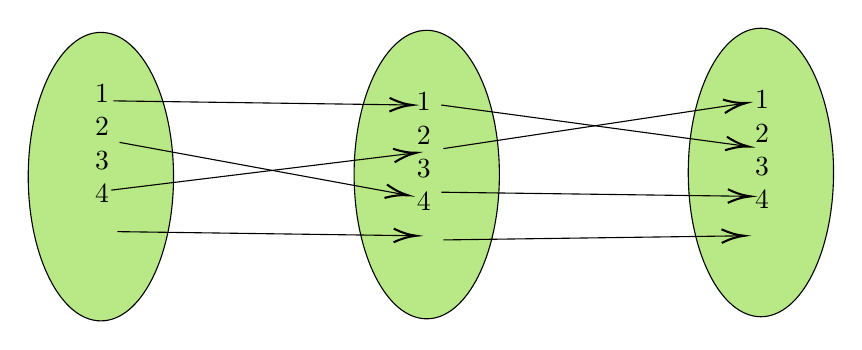
\begin{tikzpicture}[x=0.75pt,y=0.75pt,yscale=-1,xscale=1]
%uncomment if require: \path (0,300); %set diagram left start at 0, and has height of 300

%Shape: Ellipse [id:dp2987594270438807] 
\draw  [fill={rgb, 255:red, 184; green, 233; blue, 134 }  ,fill opacity=1 ] (123,81.5) .. controls (123,43.12) and (138.67,12) .. (158,12) .. controls (177.33,12) and (193,43.12) .. (193,81.5) .. controls (193,119.88) and (177.33,151) .. (158,151) .. controls (138.67,151) and (123,119.88) .. (123,81.5) -- cycle ;
%Shape: Ellipse [id:dp720654063417854] 
\draw  [fill={rgb, 255:red, 184; green, 233; blue, 134 }  ,fill opacity=1 ] (280,80.5) .. controls (280,42.12) and (295.67,11) .. (315,11) .. controls (334.33,11) and (350,42.12) .. (350,80.5) .. controls (350,118.88) and (334.33,150) .. (315,150) .. controls (295.67,150) and (280,118.88) .. (280,80.5) -- cycle ;
%Shape: Ellipse [id:dp31476275078509364] 
\draw  [fill={rgb, 255:red, 184; green, 233; blue, 134 }  ,fill opacity=1 ] (441,79.5) .. controls (441,41.12) and (456.67,10) .. (476,10) .. controls (495.33,10) and (511,41.12) .. (511,79.5) .. controls (511,117.88) and (495.33,149) .. (476,149) .. controls (456.67,149) and (441,117.88) .. (441,79.5) -- cycle ;
%Straight Lines [id:da4566390951359405] 
\draw    (164,45) -- (306,46.97) ;
\draw [shift={(308,47)}, rotate = 180.8] [color={rgb, 255:red, 0; green, 0; blue, 0 }  ][line width=0.75]    (10.93,-3.29) .. controls (6.95,-1.4) and (3.31,-0.3) .. (0,0) .. controls (3.31,0.3) and (6.95,1.4) .. (10.93,3.29)   ;
%Straight Lines [id:da44283165123573043] 
\draw    (167,65) -- (304.03,90.14) ;
\draw [shift={(306,90.5)}, rotate = 190.4] [color={rgb, 255:red, 0; green, 0; blue, 0 }  ][line width=0.75]    (10.93,-3.29) .. controls (6.95,-1.4) and (3.31,-0.3) .. (0,0) .. controls (3.31,0.3) and (6.95,1.4) .. (10.93,3.29)   ;
%Straight Lines [id:da5249229935691679] 
\draw    (163,88) -- (308.01,70.24) ;
\draw [shift={(310,70)}, rotate = 173.02] [color={rgb, 255:red, 0; green, 0; blue, 0 }  ][line width=0.75]    (10.93,-3.29) .. controls (6.95,-1.4) and (3.31,-0.3) .. (0,0) .. controls (3.31,0.3) and (6.95,1.4) .. (10.93,3.29)   ;
%Straight Lines [id:da12643161900571553] 
\draw    (166,108) -- (308,109.97) ;
\draw [shift={(310,110)}, rotate = 180.8] [color={rgb, 255:red, 0; green, 0; blue, 0 }  ][line width=0.75]    (10.93,-3.29) .. controls (6.95,-1.4) and (3.31,-0.3) .. (0,0) .. controls (3.31,0.3) and (6.95,1.4) .. (10.93,3.29)   ;
%Straight Lines [id:da9527147569060046] 
\draw    (322,47) -- (468.02,66.73) ;
\draw [shift={(470,67)}, rotate = 187.7] [color={rgb, 255:red, 0; green, 0; blue, 0 }  ][line width=0.75]    (10.93,-3.29) .. controls (6.95,-1.4) and (3.31,-0.3) .. (0,0) .. controls (3.31,0.3) and (6.95,1.4) .. (10.93,3.29)   ;
%Straight Lines [id:da8123344339093972] 
\draw    (323,68) -- (467.02,46.3) ;
\draw [shift={(469,46)}, rotate = 171.43] [color={rgb, 255:red, 0; green, 0; blue, 0 }  ][line width=0.75]    (10.93,-3.29) .. controls (6.95,-1.4) and (3.31,-0.3) .. (0,0) .. controls (3.31,0.3) and (6.95,1.4) .. (10.93,3.29)   ;
%Straight Lines [id:da3313106573539726] 
\draw    (322,89) -- (469,90.97) ;
\draw [shift={(471,91)}, rotate = 180.77] [color={rgb, 255:red, 0; green, 0; blue, 0 }  ][line width=0.75]    (10.93,-3.29) .. controls (6.95,-1.4) and (3.31,-0.3) .. (0,0) .. controls (3.31,0.3) and (6.95,1.4) .. (10.93,3.29)   ;
%Straight Lines [id:da8382142069066112] 
\draw    (323,112) -- (466,110.03) ;
\draw [shift={(468,110)}, rotate = 179.21] [color={rgb, 255:red, 0; green, 0; blue, 0 }  ][line width=0.75]    (10.93,-3.29) .. controls (6.95,-1.4) and (3.31,-0.3) .. (0,0) .. controls (3.31,0.3) and (6.95,1.4) .. (10.93,3.29)   ;

% Text Node
\draw (154,36) node [anchor=north west][inner sep=0.75pt]   [align=left] {1\\2\\3\\4};
% Text Node
\draw (309,40) node [anchor=north west][inner sep=0.75pt]   [align=left] {1\\2\\3\\4};
% Text Node
\draw (472,39) node [anchor=north west][inner sep=0.75pt]   [align=left] {1\\2\\3\\4};


\end{tikzpicture}

    \end{center}
	\begin{center}
		

\tikzset{every picture/.style={line width=0.75pt}} %set default line width to 0.75pt        

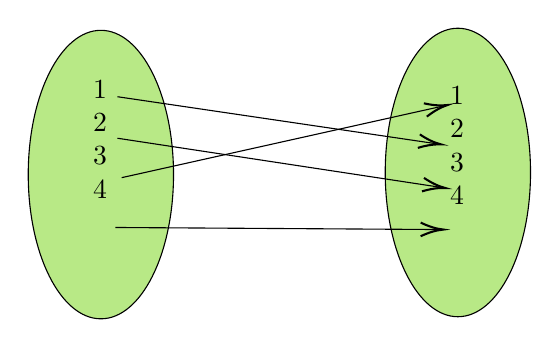
\begin{tikzpicture}[x=0.75pt,y=0.75pt,yscale=-1,xscale=1]
%uncomment if require: \path (0,300); %set diagram left start at 0, and has height of 300

%Shape: Ellipse [id:dp2987594270438807] 
\draw  [fill={rgb, 255:red, 184; green, 233; blue, 134 }  ,fill opacity=1 ] (212,82.5) .. controls (212,44.12) and (227.67,13) .. (247,13) .. controls (266.33,13) and (282,44.12) .. (282,82.5) .. controls (282,120.88) and (266.33,152) .. (247,152) .. controls (227.67,152) and (212,120.88) .. (212,82.5) -- cycle ;
%Shape: Ellipse [id:dp31476275078509364] 
\draw  [fill={rgb, 255:red, 184; green, 233; blue, 134 }  ,fill opacity=1 ] (384,81.5) .. controls (384,43.12) and (399.67,12) .. (419,12) .. controls (438.33,12) and (454,43.12) .. (454,81.5) .. controls (454,119.88) and (438.33,151) .. (419,151) .. controls (399.67,151) and (384,119.88) .. (384,81.5) -- cycle ;
%Straight Lines [id:da20444944969658452] 
\draw    (255,45) -- (409.02,67.71) ;
\draw [shift={(411,68)}, rotate = 188.39] [color={rgb, 255:red, 0; green, 0; blue, 0 }  ][line width=0.75]    (10.93,-3.29) .. controls (6.95,-1.4) and (3.31,-0.3) .. (0,0) .. controls (3.31,0.3) and (6.95,1.4) .. (10.93,3.29)   ;
%Straight Lines [id:da6452630763860843] 
\draw    (255,65) -- (411.02,88.7) ;
\draw [shift={(413,89)}, rotate = 188.64] [color={rgb, 255:red, 0; green, 0; blue, 0 }  ][line width=0.75]    (10.93,-3.29) .. controls (6.95,-1.4) and (3.31,-0.3) .. (0,0) .. controls (3.31,0.3) and (6.95,1.4) .. (10.93,3.29)   ;
%Straight Lines [id:da7747228867350222] 
\draw    (257,84) -- (412.05,49.44) ;
\draw [shift={(414,49)}, rotate = 167.43] [color={rgb, 255:red, 0; green, 0; blue, 0 }  ][line width=0.75]    (10.93,-3.29) .. controls (6.95,-1.4) and (3.31,-0.3) .. (0,0) .. controls (3.31,0.3) and (6.95,1.4) .. (10.93,3.29)   ;
%Straight Lines [id:da06374013912485954] 
\draw    (254,108) -- (410,108.99) ;
\draw [shift={(412,109)}, rotate = 180.36] [color={rgb, 255:red, 0; green, 0; blue, 0 }  ][line width=0.75]    (10.93,-3.29) .. controls (6.95,-1.4) and (3.31,-0.3) .. (0,0) .. controls (3.31,0.3) and (6.95,1.4) .. (10.93,3.29)   ;

% Text Node
\draw (242,36) node [anchor=north west][inner sep=0.75pt]   [align=left] {1\\2\\3\\4};
% Text Node
\draw (414,39) node [anchor=north west][inner sep=0.75pt]   [align=left] {1\\2\\3\\4};


\end{tikzpicture}

	\end{center}
	\begin{remark}
		The functions 
f and g are 
composed to 
yield a new 
composite 
function $g\circ f$
	\end{remark}
\end{example}

\begin{theorem}
	Let f:A$\to$B,g:$B\to C$,and h:$C\to D$.Then
	\begin{enumerate}
		\item The composition of mappings is associative;that is,$(h\circ g)\circ f=h\circ(g\circ)$
		\item If f and g are both one-to-one,them the mapping $g\circ f$is one-to-one;
		\item If f and g are both onto,then mapping $g\circ f$ is onto;
		\item If f and g are bijective,then so is $g\circ f$.
		     
	\end{enumerate}
\end{theorem}
\begin{theorem}
	A mapping is invertible if and obly if it is both one-to-one and onto.
\end{theorem}

\section{Cartesian products}

\begin{definition}
	Given sets X and Y,the CAresian product of the 
	sets X and Y,denoted by $x\times Y$,is the set of all ordered pairs(a,b) with a in X and b in Y.  
\end{definition}
\begin{note}
	The cartesian product $X_1\times X_2\times \cdots \times X_n$ of the sets $X_1,X_2,\cdots,x_n$ consists of all n-tuples$(a_1,a_2,\cdots,a_n)$with$a_i in X_i$for i=1,2,...,n.If $X=X_1=X_2=\cdots=X_n$ their Cartesian product is simply written as $X^n$
\end{note}
	
\newpage

\begin{introduction}[Keywords]
    \item  binay relation 
    \item homogeneous
    \item n-ary
    \item reflexive
    \item symmetric
    \item transitive
    \item  preorder
    \item  ineflexive
    \item asymmetric
    \item total
    \item antisymmetric
    \item complete
    \item poset
    \item relatively prime
    \item quasi prder
    \item partial order
    \item total order
    \item chain 
    \item minimum
    \item maximum
    \item minimal
    \item partition
    \item equivalence relation
    \item equivalence class
    \item quotient
    \item tolerance relation
    \item singleton
\end{introduction}
\section{Binary relation}

\begin{definition}[binary]
\begin{enumerate}
	\item 	A binary operation on a nonempty set A is a mapping.be written as $A\times A\to A$
	\item A binary operation * on A is associative if (ab)c=a(bc) for all abc$\in$ A
	\item A binary operation * on A is comunative of ab=ba for all abc$\in$ A
\end{enumerate}
\end{definition}

\begin{definition}[identity]
Let *:A$\times A \to $be a binary operation A
\begin{enumerate}
	\item if\quad l$\in$A,la=a\quad l is left identity
	\item if\quad l$\in$A,al=a\quad l is right identity
	\item if\quad l$\in$A,al=la=a\quad l is identity
\end{enumerate}	
\end{definition}

\begin{theorem}
	if  l and r respectively left and right identity in A,then l = r is an identity
\end{theorem}
	
\begin{theorem}
	The identity is unique in A if it exist.
\end{theorem}
\begin{proof}
	Assume A has more than a identity,$e_1,e_2,\cdots,e_n$\\
	we know :
\begin{align*}
	&e_1=e_1\cdot e_2=e_2\\	
	&e_3=e_2\cdot e_3=e_3\\
	&\vdots\\
	&e_{n-1}=e_{n-1}\cdot e_n=e_n
\end{align*}
so $e_1=e_2=\cdots=e_n$,the identity is only one,if it exists.
\end{proof}
\begin{definition}
    Let R be a binary relation between A and B. If (a,b) $\in$ R, then we say that a is R-related to b (or a, b are R-related), which is denoted by a R b. 
\end{definition}
\begin{remark}
    The domain of R is the set of all x $\in$ A such that x R y for some
y $\in$ B. The range of R is the set of all y $\in$ B such that x R y for some x $\in$ A.
\end{remark}

\\
\begin{example}
    Let A={Gardner, Valerian, Olivia, Frank, Daisy} and
B={London, Berlin, Paris, Boston}. Suppose that: 
\begin{enumerate}
    \item Gardner and Valerian were born in London;
    \item Olivia was born in Boston;
    \item Frank and Daisy were born in Paris.
\end{enumerate}
\end{example}
\begin{proof}
    The above information can be described in terms of a binary relation R given by:
\begin{equation*}
    R={(Gardner, London), (Valerian, London),
(Olivia, Boston), (Frank, Paris), (Daisy, Paris)}
\end{equation*}
\end{proof}

\begin{property}
    A binary relation R on A is said to be:
\begin{itemize}
    \item reflexive $\Leftrightarrow \forall$$ x $\in $A, x R x.
    \item irreflexive (or strict) $\Leftrightarrow \forall$ $ x \in $A, ¬(x R x)
    \item symmetric$ \Leftrightarrow \forall $x, y $\in$ A, x R y$ \Rightarrow$ y R x.
    \item antisymmetric $\Leftrightarrow \forall$ x, y \in A, (x R y)$ \land$ $ (y R x) \Rightarrow$ x=y
    \item  asymmetric $\Leftrightarrow \forall$ x, y $\in$ A, x R y $\Leftrightarrow$ ¬(y R x).
    \item transitive$\Leftrightarrow \forall$ x, y,Z \in A, (x R y) $\land$ (y R z) $\Rightarrow$ x R z.
    \item  complete $\Leftrightarrow \froall$x, y $\in$ A, x $\neq$ y $\Rightarrow$ (x R y) $\lor$ (y R x).
    \item total (or strong complete) $\Leftrightarrow$ $\forall$x, y $\in$ A, (x R y) $\lor$ (y R x).

\end{itemize}

\end{property}

\begin{example}
    \begin{enumerate}
        \item The relations =, $\leq$ and $\ge$ are reflexive.
        \item The relations $\textless$ and $\textgreater$ are irreflexive.
        \item The relations = and “relatively prime” are symmetric.

        \item The relations $\leq$ and $\ge$ are antisymmetric.
        \item The relations $\textless$ and $\textgreater$ are asymmetric.
        \item The relations =, $\leq$ and $\ge$ are transitive
        \item The relations $\textless$ and $\textgreater$  are complete but not total
        \item The relations $\leq$ and $\ge$ are total. 
        
    \end{enumerate}
\end{example}

\begin{theorem}
    Let R be a binary relation on A. Then the
following are equivalent:
\begin{enumerate}
    \item R is antisymmetric.
    \item $\forall$x,y$\in$A,(x R y)$\land$(x $\neq$ y)$\Rightarrow$$\lnot$(y R x)
\end{enumerate}
\end{theorem}
\begin{proof}
    \begin{align*}
        R is antisymmetric &\Leftrightarrow \forall x,y \in A,(x R y)\land (y R x) \rightarrow x=y\\
        & \Leftrightarrow \forall x,y \in A,(x R y)\rightarrow ((y R x) \rightarrow x=y) (CP.rule)\\
        & \Leftrightarrow \forall x,y \in A,(x R y)\rightarrow (x\neq y\rightarrow \lnot (yRx))\\
        &  \Leftrightarrow \forall x,y \in A,(x R y) \land (x \neq y)\Rightarrow \lnot (y R x)
    \end{align*}
\end{proof}
\begin{theorem}
    Let R be a binary relation on A. Then the
following are equivalent:
\begin{enumerate}
    \item R is asymmetric.
    \item  R is antisymmetric and irreflexive.
\end{enumerate}

\end{theorem}
\newpage
\begin{proof}
    \begin{enumerate}
        \item Assume that R is asymmetric,Then we have (x R y)$\Rightarrow$$\lnot$(yRx).It follows that $\forall$x,y$\in$A,(x R y)$\land$(x $\neq$ y)$\Rightarrow$$\lnot$(y R x),Thus R is antisymmetric,Let x$\in$A.since R is asymmetric,we have xRy$\rightarrow \lnot$(yRx)
        \item Assume that R is not irreflexive.Then there exists $x_0\in A$such that $x_0Rx$.It follows that $\lnot (x_0R_0x_0)$.This lead to a contradication.Therefore,R is irreflexive
        \item Assume that R is antisymmetric and irreflexive,Let XRy for x,y$\in$A,Note first that $x\neq y$since R is irreflexive thus we have $\lnot (yRx)$since R is antisiymmetric.Therefore R is antisymmetric
    \end{enumerate}
\end{proof}
\begin{proposition}
    if $P_1\Rightarrow P_2$ then $P_2\rightarrow Q \Rightarrow P_1\rightarrow Q$
\end{proposition}
\begin{proof}
    if $P_1\Rightarrow P_2$:
        \begin{align*}
            (P_2\rightarrow Q) \rightarrow (P_1 \rightarrow Q) &\Leftrightarrow \lnot(P_1\rightarrow Q)\rightarrow \lnot (P_2\rightarrow Q)\\
            &\Leftrightarrow(P_1\land \lnot Q)\rightarrow (P_2\land \lnot Q)
        \end{align*}
    Since $v(P_1)$\leq$ v(P_2),v(p_1\land \lnot Q)$\leq$v(p_2\land \lnot Q)$,Hence $P_1\Rightarrow P_2$ then $P_2\rightarrow Q \Rightarrow P_1\rightarrow Q$
\end{proof}

\begin{theorem}
    Let R be a binary relation on A. Then the
following are equivalent:
\begin{enumerate}
    \item R is complete.
    \item $\forall x,y\in A,(x=y)\lor (xRy)\lor (yRx).$
\end{enumerate}
\end{theorem}

\begin{theorem}
    Let R be a binary relation on A. Then the
following are equivalent:
\begin{enumerate}
    \item R is total.
    \item R is reflexive and complete.
\end{enumerate}
\end{theorem}
\begin{note}
    total = feflexive + complete
\end{note}
\begin{proof}
    \begin{align*}
        \underset{totoal}{(xRy)\lor (yRx)}&\Leftrightarrow((x=y)\land(x\neq y))\land (xRy)\land (yRx)\\
        &\Leftrightarrow((x=y)\rightarrow(xRy)\land(yRx))\land(x\neq y)\to (xRy)\land(yRx)\\
        &\Leftrightarrow \underset{reflexive}{((x=y)\to xRy)}\land \underset{complete}{(x\neq y \lor (xRy)\lor (yRx)}
    \end{align*}
\end{proof}
\newpage
\section{Order relation}

\begin{proposition}
    Let $\leq$ be a binary relation on A.Then we say that:
    \begin{enumerate}
        \item $\leq$ is a preorder (or quasi order)$\Leftrightarrow$$\leq$ is re flexive and transitive.
        \item $\leq$ is a weak order $\Leftrightarrow$ $\leq$ is total and transitive 
        \item $\leq$ partial order $\Leftrightarrow$ $\leq$is reflexive,antisymmetric and transitive
        \item $\leq$ is a total order$\Leftrightarrow$$\leq$ is total,antisymmetric and transive
        \item $\leq$ is a strict partial order $\Leftrightarrow$$\leq$ is irreflexive and transitive
        \item $\leq$ is a strict total order $\Leftrightarrow$ $\leq$ is irreflexive,compete and transitive 
    \end{enumerate}
    \begin{remark}
        \textcolor{red!80}{Strict total orders are not total oeders}
    \end{remark}
\end{proposition}

\begin{theorem}
    Let $\leq$ be a binary relation on A. Then the 
following are equivalent:
\begin{enumerate}
    \item $\leq$ is a partial order
    \item $\leq$ is an antisymmetric preorder.
\end{enumerate}
\end{theorem}

\begin{center}
    

\tikzset{every picture/.style={line width=0.75pt}} %set default line width to 0.75pt        

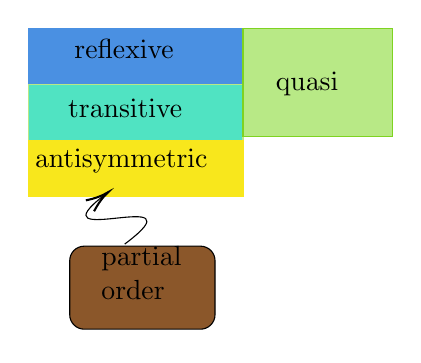
\begin{tikzpicture}[x=0.75pt,y=0.75pt,yscale=-1,xscale=1]
%uncomment if require: \path (0,448); %set diagram left start at 0, and has height of 448

%Shape: Rectangle [id:dp8061075849581709] 
\draw  [color={rgb, 255:red, 74; green, 144; blue, 226 }  ,draw opacity=1 ][fill={rgb, 255:red, 74; green, 144; blue, 226 }  ,fill opacity=1 ] (-392,42) -- (-288.5,42) -- (-288.5,69) -- (-392,69) -- cycle ;
%Shape: Rectangle [id:dp8845509569015728] 
\draw  [color={rgb, 255:red, 184; green, 233; blue, 134 }  ,draw opacity=1 ][fill={rgb, 255:red, 80; green, 227; blue, 194 }  ,fill opacity=1 ] (-392,69) -- (-288.5,69) -- (-288.5,96) -- (-392,96) -- cycle ;
%Shape: Rectangle [id:dp2723240890652203] 
\draw  [color={rgb, 255:red, 248; green, 231; blue, 28 }  ,draw opacity=1 ][fill={rgb, 255:red, 248; green, 231; blue, 28 }  ,fill opacity=1 ] (-392,96) -- (-288.5,96) -- (-288.5,123) -- (-392,123) -- cycle ;
%Flowchart: Alternative Process [id:dp9909037900604678] 
\draw  [fill={rgb, 255:red, 139; green, 87; blue, 42 }  ,fill opacity=1 ] (-372,154) .. controls (-372,150.13) and (-368.87,147) .. (-365,147) -- (-309,147) .. controls (-305.13,147) and (-302,150.13) .. (-302,154) -- (-302,180) .. controls (-302,183.87) and (-305.13,187) .. (-309,187) -- (-365,187) .. controls (-368.87,187) and (-372,183.87) .. (-372,180) -- cycle ;
%Curve Lines [id:da21055504424033877] 
\draw    (-345.5,146) .. controls (-305.9,116.3) and (-391.75,150.31) .. (-354.66,121.88) ;
\draw [shift={(-353.5,121)}, rotate = 143.13] [color={rgb, 255:red, 0; green, 0; blue, 0 }  ][line width=0.75]    (10.93,-3.29) .. controls (6.95,-1.4) and (3.31,-0.3) .. (0,0) .. controls (3.31,0.3) and (6.95,1.4) .. (10.93,3.29)   ;
%Shape: Rectangle [id:dp7180759333454068] 
\draw  [color={rgb, 255:red, 126; green, 211; blue, 33 }  ,draw opacity=1 ][fill={rgb, 255:red, 184; green, 233; blue, 134 }  ,fill opacity=1 ] (-288.5,42) -- (-216.5,42) -- (-216.5,94) -- (-288.5,94) -- cycle ;

% Text Node
\draw (-366,49.4) node [anchor=north west][inner sep=0.75pt]    {$$};
% Text Node
\draw (-371,46) node [anchor=north west][inner sep=0.75pt]   [align=left] {reflexive\\};
% Text Node
\draw (-374,75) node [anchor=north west][inner sep=0.75pt]   [align=left] {transitive\\};
% Text Node
\draw (-390,99) node [anchor=north west][inner sep=0.75pt]   [align=left] {antisymmetric\\};
% Text Node
\draw (-358,146) node [anchor=north west][inner sep=0.75pt]   [align=left] {partial \\order\\};
% Text Node
\draw (-274,62) node [anchor=north west][inner sep=0.75pt]   [align=left] {quasi\\};


\end{tikzpicture}

\end{center}

\begin{theorem}
    Let $\leq$ be a binary relation on A.then:
    \begin{enumerate}
        \item $\leq$ is a weak order
        \item $\leq$ is a complete preorder
    \end{enumerate}
\end{theorem}
\begin{proof}
    \begin{align*}
        &\Leftrightarrow \text{R is a complete,reflexive and transitive}\\
        &\Leftrightarrow \text{R is total and transitive} \\
        &\Leftrightarrow \text{R is weak order}
    \end{align*}
\end{proof}

\begin{center}
    


\tikzset{every picture/.style={line width=0.75pt}} %set default line width to 0.75pt        

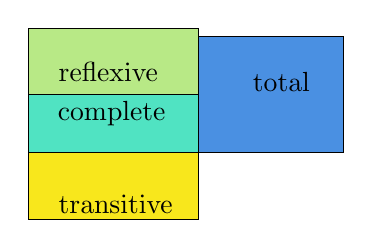
\begin{tikzpicture}[x=0.75pt,y=0.75pt,yscale=-1,xscale=1]
%uncomment if require: \path (0,448); %set diagram left start at 0, and has height of 448

%Shape: Rectangle [id:dp18641892582068387] 
\draw  [fill={rgb, 255:red, 184; green, 233; blue, 134 }  ,fill opacity=1 ] (280,126) -- (362,126) -- (362,158) -- (280,158) -- cycle ;
%Shape: Rectangle [id:dp32615047594152813] 
\draw  [fill={rgb, 255:red, 80; green, 227; blue, 194 }  ,fill opacity=1 ] (280,158) -- (362,158) -- (362,190) -- (280,190) -- cycle ;
%Shape: Rectangle [id:dp8023157172561419] 
\draw  [fill={rgb, 255:red, 248; green, 231; blue, 28 }  ,fill opacity=1 ] (280,186) -- (362,186) -- (362,218) -- (280,218) -- cycle ;
%Shape: Rectangle [id:dp5404533522876682] 
\draw  [fill={rgb, 255:red, 74; green, 144; blue, 226 }  ,fill opacity=1 ] (362,130) -- (432,130) -- (432,186) -- (362,186) -- cycle ;

% Text Node
\draw (293,160) node [anchor=north west][inner sep=0.75pt]   [align=left] {complete\\};
% Text Node
\draw (340,155) node   [align=left] {\begin{minipage}[lt]{68pt}\setlength\topsep{0pt}
reflexive\\
\end{minipage}};
% Text Node
\draw (387,146) node [anchor=north west][inner sep=0.75pt]   [align=left] {total\\};
% Text Node
\draw (340,211) node   [align=left] {\begin{minipage}[lt]{68pt}\setlength\topsep{0pt}
transitive
\end{minipage}};


\end{tikzpicture}
\end{center}
\newpage
\begin{theorem}
    Let $\leq$ be a binary relation on A,Then:
    \begin{enumerate}
        \item $\leq$ is a total order
        \item $\leq$ is a complete partial order
        \item $\leq$ is an antisymmetric weak order
    \end{enumerate}
\end{theorem}


\begin{center}
    

\tikzset{every picture/.style={line width=0.75pt}} %set default line width to 0.75pt        

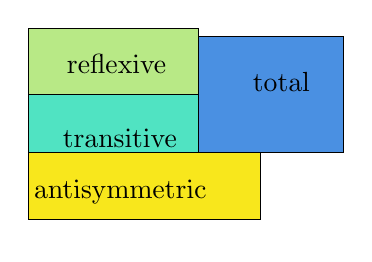
\begin{tikzpicture}[x=0.75pt,y=0.75pt,yscale=-1,xscale=1]
%uncomment if require: \path (0,448); %set diagram left start at 0, and has height of 448

%Shape: Rectangle [id:dp18641892582068387] 
\draw  [fill={rgb, 255:red, 184; green, 233; blue, 134 }  ,fill opacity=1 ] (280,126) -- (362,126) -- (362,158) -- (280,158) -- cycle ;
%Shape: Rectangle [id:dp32615047594152813] 
\draw  [fill={rgb, 255:red, 80; green, 227; blue, 194 }  ,fill opacity=1 ] (280,158) -- (362,158) -- (362,190) -- (280,190) -- cycle ;
%Shape: Rectangle [id:dp8023157172561419] 
\draw  [fill={rgb, 255:red, 248; green, 231; blue, 28 }  ,fill opacity=1 ] (280,186) -- (392,186) -- (392,218) -- (280,218) -- cycle ;
%Shape: Rectangle [id:dp5404533522876682] 
\draw  [fill={rgb, 255:red, 74; green, 144; blue, 226 }  ,fill opacity=1 ] (362,130) -- (432,130) -- (432,186) -- (362,186) -- cycle ;

% Text Node
\draw (281.39,198) node [anchor=north west][inner sep=0.75pt]  [xslant=-0.02] [align=left] {antisymmetric\\};
% Text Node
\draw (344,151) node   [align=left] {\begin{minipage}[lt]{68pt}\setlength\topsep{0pt}
reflexive\\
\end{minipage}};
% Text Node
\draw (387,146) node [anchor=north west][inner sep=0.75pt]   [align=left] {total\\};
% Text Node
\draw (342,179) node   [align=left] {\begin{minipage}[lt]{68pt}\setlength\topsep{0pt}
transitive
\end{minipage}};


\end{tikzpicture}

\end{center}

\begin{note}
    \begin{center}
        

\tikzset{every picture/.style={line width=0.75pt}} %set default line width to 0.75pt        

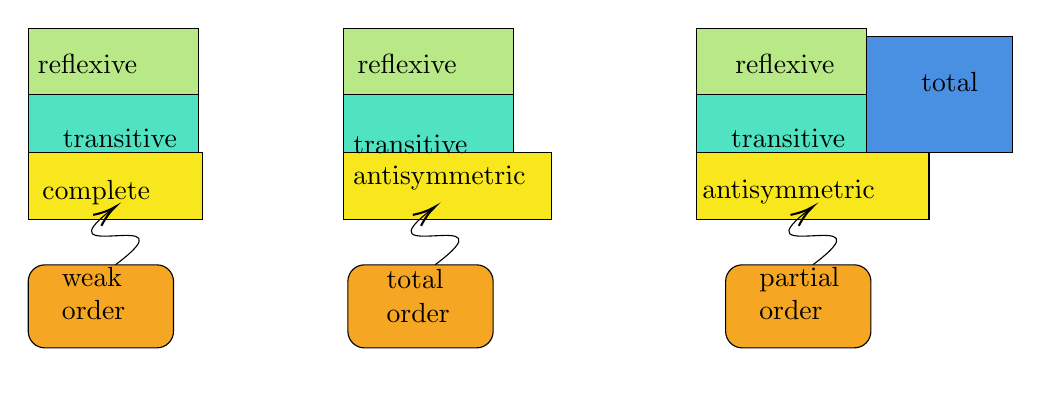
\begin{tikzpicture}[x=0.75pt,y=0.75pt,yscale=-1,xscale=1]
%uncomment if require: \path (0,448); %set diagram left start at 0, and has height of 448

%Shape: Rectangle [id:dp18641892582068387] 
\draw  [fill={rgb, 255:red, 184; green, 233; blue, 134 }  ,fill opacity=1 ] (532,112) -- (614,112) -- (614,144) -- (532,144) -- cycle ;
%Shape: Rectangle [id:dp32615047594152813] 
\draw  [fill={rgb, 255:red, 80; green, 227; blue, 194 }  ,fill opacity=1 ] (532,144) -- (614,144) -- (614,176) -- (532,176) -- cycle ;
%Shape: Rectangle [id:dp8023157172561419] 
\draw  [fill={rgb, 255:red, 248; green, 231; blue, 28 }  ,fill opacity=1 ] (532,172) -- (644,172) -- (644,204) -- (532,204) -- cycle ;
%Shape: Rectangle [id:dp5404533522876682] 
\draw  [fill={rgb, 255:red, 74; green, 144; blue, 226 }  ,fill opacity=1 ] (614,116) -- (684,116) -- (684,172) -- (614,172) -- cycle ;
%Shape: Rectangle [id:dp1281581580329123] 
\draw  [fill={rgb, 255:red, 184; green, 233; blue, 134 }  ,fill opacity=1 ] (210,112) -- (292,112) -- (292,144) -- (210,144) -- cycle ;
%Shape: Rectangle [id:dp5575594363799885] 
\draw  [fill={rgb, 255:red, 80; green, 227; blue, 194 }  ,fill opacity=1 ] (210,144) -- (292,144) -- (292,176) -- (210,176) -- cycle ;
%Shape: Rectangle [id:dp4319095317678616] 
\draw  [fill={rgb, 255:red, 248; green, 231; blue, 28 }  ,fill opacity=1 ] (210,172) -- (294,172) -- (294,204) -- (210,204) -- cycle ;
%Shape: Rectangle [id:dp7826861943215782] 
\draw  [fill={rgb, 255:red, 184; green, 233; blue, 134 }  ,fill opacity=1 ] (362,112) -- (444,112) -- (444,144) -- (362,144) -- cycle ;
%Shape: Rectangle [id:dp47008145861553574] 
\draw  [fill={rgb, 255:red, 80; green, 227; blue, 194 }  ,fill opacity=1 ] (362,144) -- (444,144) -- (444,176) -- (362,176) -- cycle ;
%Shape: Rectangle [id:dp6477705342064104] 
\draw  [fill={rgb, 255:red, 248; green, 231; blue, 28 }  ,fill opacity=1 ] (362,172) -- (462,172) -- (462,204) -- (362,204) -- cycle ;
%Curve Lines [id:da4458005287285718] 
\draw    (252,226) .. controls (291.6,196.3) and (213.59,227.37) .. (250.84,198.88) ;
\draw [shift={(252,198)}, rotate = 143.13] [color={rgb, 255:red, 0; green, 0; blue, 0 }  ][line width=0.75]    (10.93,-3.29) .. controls (6.95,-1.4) and (3.31,-0.3) .. (0,0) .. controls (3.31,0.3) and (6.95,1.4) .. (10.93,3.29)   ;
%Rounded Rect [id:dp8181002178799672] 
\draw  [fill={rgb, 255:red, 245; green, 166; blue, 35 }  ,fill opacity=1 ] (210,234) .. controls (210,229.58) and (213.58,226) .. (218,226) -- (272,226) .. controls (276.42,226) and (280,229.58) .. (280,234) -- (280,258) .. controls (280,262.42) and (276.42,266) .. (272,266) -- (218,266) .. controls (213.58,266) and (210,262.42) .. (210,258) -- cycle ;
%Curve Lines [id:da08373613929158363] 
\draw    (406,226) .. controls (445.6,196.3) and (367.59,227.37) .. (404.84,198.88) ;
\draw [shift={(406,198)}, rotate = 143.13] [color={rgb, 255:red, 0; green, 0; blue, 0 }  ][line width=0.75]    (10.93,-3.29) .. controls (6.95,-1.4) and (3.31,-0.3) .. (0,0) .. controls (3.31,0.3) and (6.95,1.4) .. (10.93,3.29)   ;
%Rounded Rect [id:dp771691938533626] 
\draw  [fill={rgb, 255:red, 245; green, 166; blue, 35 }  ,fill opacity=1 ] (364,234) .. controls (364,229.58) and (367.58,226) .. (372,226) -- (426,226) .. controls (430.42,226) and (434,229.58) .. (434,234) -- (434,258) .. controls (434,262.42) and (430.42,266) .. (426,266) -- (372,266) .. controls (367.58,266) and (364,262.42) .. (364,258) -- cycle ;
%Curve Lines [id:da6472855674062663] 
\draw    (588,226) .. controls (627.6,196.3) and (549.59,227.37) .. (586.84,198.88) ;
\draw [shift={(588,198)}, rotate = 143.13] [color={rgb, 255:red, 0; green, 0; blue, 0 }  ][line width=0.75]    (10.93,-3.29) .. controls (6.95,-1.4) and (3.31,-0.3) .. (0,0) .. controls (3.31,0.3) and (6.95,1.4) .. (10.93,3.29)   ;
%Rounded Rect [id:dp06886982283668308] 
\draw  [fill={rgb, 255:red, 245; green, 166; blue, 35 }  ,fill opacity=1 ] (546,234) .. controls (546,229.58) and (549.58,226) .. (554,226) -- (608,226) .. controls (612.42,226) and (616,229.58) .. (616,234) -- (616,258) .. controls (616,262.42) and (612.42,266) .. (608,266) -- (554,266) .. controls (549.58,266) and (546,262.42) .. (546,258) -- cycle ;

% Text Node
\draw (533.39,184) node [anchor=north west][inner sep=0.75pt]  [xslant=-0.02] [align=left] {antisymmetric\\};
% Text Node
\draw (596,137) node   [align=left] {\begin{minipage}[lt]{68pt}\setlength\topsep{0pt}
reflexive\\
\end{minipage}};
% Text Node
\draw (639,132) node [anchor=north west][inner sep=0.75pt]   [align=left] {total\\};
% Text Node
\draw (594,165) node   [align=left] {\begin{minipage}[lt]{68pt}\setlength\topsep{0pt}
transitive
\end{minipage}};
% Text Node
\draw (215.39,184) node [anchor=north west][inner sep=0.75pt]  [xslant=-0.02] [align=left] {complete\\};
% Text Node
\draw (260,137) node   [align=left] {\begin{minipage}[lt]{68pt}\setlength\topsep{0pt}
reflexive\\
\end{minipage}};
% Text Node
\draw (272,165) node   [align=left] {\begin{minipage}[lt]{68pt}\setlength\topsep{0pt}
transitive
\end{minipage}};
% Text Node
\draw (365.08,177) node [anchor=north west][inner sep=0.75pt]  [xslant=-0.02] [align=left] {antisymmetric\\\\};
% Text Node
\draw (414,137) node   [align=left] {\begin{minipage}[lt]{68pt}\setlength\topsep{0pt}
reflexive\\
\end{minipage}};
% Text Node
\draw (412,168) node   [align=left] {\begin{minipage}[lt]{68pt}\setlength\topsep{0pt}
transitive
\end{minipage}};
% Text Node
\draw (225,226) node [anchor=north west][inner sep=0.75pt]   [align=left] {weak\\order\\};
% Text Node
\draw (428,249) node   [align=left] {\begin{minipage}[lt]{68pt}\setlength\topsep{0pt}
total\\order\\
\end{minipage}};
% Text Node
\draw (561,226) node [anchor=north west][inner sep=0.75pt]   [align=left] {partial\\order\\};


\end{tikzpicture}

    \end{center}
\end{note}

\section{Equivalence relation}
\begin{theorem}
A binary relation R on A is called an equivalence
relation if it is reflexive, symmetric and transitive. For a $\in$ A,
the set $[a]_R$=$\{ b \in A | a R b \}$ is called the equivalence class of a under R.
\end{theorem}
\begin{example}
    \footnote{A first course in Abstract algebra.98}The equivalence class of (a,b) under cross-multiplication, where a,b$\in Z$
and b $\neq$ 0,is:
\begin{equation*}
    [(a,b)]=\{(c,d):ad = bc\}
\end{equation*}
If we denote [(a,b)] by a/b, then this equivalence class is precisely the
fraction usually denoted by a=b. After all, it is plain that (1,2)$\neq$(2,4),
but [(1,2)]=[(2,4)]; that is, $\frac{1}{2}=\frac{2}{4}$
\end{example}
\begin{example}
    An equivalence class[(P,Q)] of arrows, as in Example 2.17(iv), is called
a vector; we denote it by [(P,Q)]=$\overrightarrow{PQ}$
\end{example}
\begin{lemma}
If $\equiv$ is an equivalence relation on a set X, then x $\equiv$ y if and
only if [x]=[y].
\end{lemma}

\begin{proof}
    Assume that x$\equiv$ y. If z $\in$[x], then z$\equiv$x, and so transitivity gives
z $\equiv$y; hence [x]⊆ [y]. By symmetry, y$\equiv$ x, and this gives the reverse
inclusion[y]$\subseteq $ [x]. Thus, [x]=[y]
Conversely, if [x]= [y], then x $\in$ [x], by reflexivity, and so x $\in$ [x] = [y].
Therefore, x $\equiv$ y
\end{proof}

\begin{theorem}
    Let R be an equivalence relation on A. Then 
    \begin{equation*}
        A/R=\{[a]_R|a\in A\}
    \end{equation*}
    is called the quotient set of A by R.
\end{theorem}
\begin{theorem}
    Let R be an equivalence relation on A. Then
the following are equivalent:
\begin{enumerate}
    \item a R b
    \item $b\in [a]_R$
    \item $[a]_R=[b]_R$
\end{enumerate}
\end{theorem}


\begin{definition}
     Let R be an equivalence relation on A. Then 
either $[a]_R$ = $[b]_R$ or $[a]_R$ $\cap$ $[b]_R$ = $\emptyset$ for all a,b $\in$ A.
\end{definition}
\begin{note}
   \footnote{A first course in Abstract algebra.99} A partition of a set X is a family of nonempty pairwise disjoint subsets,
called blocks, whose union is all of X.
Notice that if X is a finite set and $A_1,A2,\dots,A_n$ is a partition of X, then
\begin{equation*}
    |X|=|A_1|+|A_2|+\cdots+|A_n|
\end{equation*}
\end{note}
We are now going to prove that equivalence relations and partitions are
merely different views of the same thing
\begin{proposition}
    If $\equiv$ is an equivalence relation on a set X, then the equivalence classes form a partition P of X. Conversely, given a partition of X, there
is an equivalence relation on X whose equivalence classes are the blocks in P.
\end{proposition}
\begin{proof}
    \footnote{A first course in Abstract algebra.99}Assume that an equivalence relation $\equiv$ on X is given. Each x $\in$ X lies
in the equivalence class [x] because $\equiv$is reflexive; it follows that the equivalence
classes are nonempty subsets whose union is X. To prove pairwise disjointness,
assume that a $\in$ [x] $\cap$ [y], so that a $\equiv$x and a $\equiv$y. By symmetry, x $\equiv$a,
and so transitivity gives x $\equiv$y. Therefore,[x] = [y], by the lemma, and so the equivalence classes form a partition of X.
\\
Conversely, let P be a partition of X. If x,y$\in$X, define x $\equiv$y if there is
A $\in$ P with x $\in$ A and y $\in$ A. It is plain that $\equiv$is reflexive and symmetric. To
see that $\equiv$is transitive, assume that x $\equiv$y and y $\equiv$z; that is, there are A,B$\in$ P
with x, y $\in$ A and y, z $\in$ B. Since y $\in$ A\ B, pairwise disjointness gives A D B
and so x, z $\in$ A; that is, x $\equiv$z. We have shown that $\equiv$is an equivalence relation.
\\
It remains to show that the equivalence classes are the subsets in P . If x $\in$ X,
then x $\in$ A for some A $\in$ P. By definition of ≡, if y $\in$ A, then y $\equiv$x
and y $\in$ [x]; hence, A $\subseteq$[x]. For the reverse inclusion, let z $\in$ [x], so that
z $\equiv$x. There is some B with x $\in$ B and z $\in$ B; thus, x $\in$ A $\cap$ B. By pairwise
disjointness, A = B, so that z $\in$ A, and [x] $\subseteq$ A. Hence, [x]=A. •
\end{proof}
\begin{definition}
     Let R be an equivalence relation on A. Then $\cap$$\{ [a]_R| a $$\in A \}$ = A
\end{definition}

\newpage
\section{Partitions}
\begin{definition}
    Let A be a nonempty set and P = $\{$A_i$ | i $\in$ I\}$ be a
family of subsets of A such that
\begin{enumerate}
    \item $\forall i \in I,A_i \neq \emptyset$
    \item $\cap \{A_i|i\in I\}$=A
    \item $A_i\neq A_j\Rightarrow A_i\cap A_j=\emptyset$
\end{enumerate}
 Then P is called a partition of A
\end{definition}

\begin{theorem}
    Let R be an equivalence relation on A. Then
    \begin{equation*}
        A/R=\{[a]_R|a\in A\}
    \end{equation*}
    forms a partion of A
\end{theorem}

\begin{theorem}
     Let P = $\{A_i | i \in I\}$ be a partition of A. Then the
binary relation R on A given by
\begin{equation*}
    a R b \Leftrightarrow \exists i \in I,\{a,b\}\subseteq A_i
\end{equation*}
is an equivalence relation on A.
\end{theorem}

\section{Division}

\begin{definition}
    If a and b are integers, then a is a divisor(or \textbf{factor}) of b if there is an integer d with b = ad (synonyms are a divides b and also b is a \textbf{multiple} of a). We denote this by:
    \begin{equation*}
        a|b
    \end{equation*}
\end{definition}
\begin{proof}
    Note that 3$|$6, because 6 = 3×2, but that 3$|$5 (that is, 3 does not divide 5):even though 5 = 3 × 5=$\frac{5}{3}\times 3$,the fraction$\frac{5}{3}$is not an integer.
\end{proof}

\begin{definition}
    A common divisor of integers a and b is an integer c with c$ | $a and $c | b$. \textbf{The greatest common divisor} of a and b, denoted by gcd(a, b) [or, more briefly, by (a, b)], is defined by:
    \begin{equation*}
        gdc(a,b)=\begin{cases}
        0\quad if a=0=b\\
       \text{the largest common divisor of a and b otherwise.}
        \end{cases}
    \end{equation*}
\end{definition}
\begin{note}
    The notation (a, b) for the gcd is, obviously, the same notation used for the ordered pair. The reader should have no difficulty understanding the intended meaning from the context in which the symbol occurs.
\end{note}
\begin{note}
    
    \begin{itemize}
        \item If a and m are positive integers with $a | m$, say, m = ab, we claim that $a \leq m$. Since $0\textless b$, we have 1 ≤ b, because b is an integer, and so a $\leq$ ab = m. It follows that gcd’s always exist.
        \item If c is a common divisor of a and b,then so is −c. Since one of $\sqrt{m}$ c is non negative, the gcd is always nonnegative. It is easy to check that if at least one of a and b is nonzero, then (a,b)$\textgreater$0.
    \end{itemize}
\end{note}

\begin{proposition}
    if p is a prime and b is any integer, then:
    \begin{equation*}
        (p.b)=\begin{cases}
            \text{p if $p|b$}\\
            \text{1 otherwise.}
            \end{cases}
    \end{equation*}
    
\end{proposition}
\begin{proof}
A common divisor c of p and a is, of course, a divisor of p. But the only positive divisors of p are p and 1, and so (p,a) = p or 1; it is p if $p| a$, and it is 1 otherwise.
\end{proof}



\begin{definition}
    Let $a_1,\cdots,a_n$ be positive integers. 
The smallest positive integer m which is 
$divisible by all $$a_i$ $(i=1,\cdots,n)$, is called the least common multiple of $a_1,\cdots,a_n$, and is denoted by $m=lcm(a_1,\cdots,a_n)$ .
\end{definition}







\begin{definition}
    

    A positive integer p greater than 1 is said to be prime if 1 and p are the only positive factors of p. An interger p$\textgreater$1 is called a composite number if it is not prime.
\end{definition}

\begin{theorem}
    Every integer n $\geq$ 2 is either a prime or a product of primes.
\end{theorem}
\begin{proof}
    Were this not so, there would be “criminals:” there are integers n $\geq$ 2 which are neither primes nor products of primes; a least criminal m is the
smallest such integer. Since m is not a prime, it is composite; there is thus a
factorization m D ab with 2 $\leq$ a $\textless$ m and 2 $\leq$b $\textless$m (since a is an integer,
1 $\textless$ a implies 2  $\leq$  a). Since m is the least criminal, both a and b are “honest,”
i.e.,\begin{equation*}
    a=pp^{'}p^{''}... \quad b=qq^{'}q^{''} ...
\end{equation*}
where the factors$a=pp^{'}p^{''}... \quad b=qq^{'}q^{''} ...$are primes.Therefore,
\begin{equation*}
    m=ab==pp^{'}p^{''}...qq^{'}q^{''} ...
\end{equation*}
is a product of (at least two) primes, which is a contradiction.
\end{proof}
\begin{proposition}
    If m $\geq$ 2 is a positive integer which is not divisible by any
prime p with p $\leq$ $\sqrt{m}$, then m is a prime.
\end{proposition}
\begin{proof}
    If m is not prime, then m = ab, where a $\textless$ m and b $\textless$ m are positive
integers. If a $\textgreater$ $\sqrt{m}$ and b $\textgreater$ $\sqrt{m}$, then m = ab $\textgreater$$\sqrt{m}$$\sqrt{m}$ = m, a contradiction.
Therefore, we may assume that a$\leq$ $\sqrt{m}$. By Theorem 2.17, a is either a
prime or a product of primes, and any (prime) divisor p of a is also a divisor of
m. Thus, if m is not prime, then it has a “small” prime divisor p; i.e., p$\leq$ $\sqrt{m}$.
The contrapositive says that if m has no small prime divisor, then m is prime. 
\end{proof}
\begin{note}
    can be used to show that 991 is a prime. It suffices to check
whether 991 is divisible by some prime p with p $\leq$
991 $\approx$ 31.48; if 991 isnot divisible by 2, 3, 5, ... , or 31, then it is prime.
\end{note}

\begin{definition}
    Two integers are relatively primeif their greatest common divisor is 1. The integers $a_1,…,a_n$ are pairwise relatively prime if gcd($a_i, a_j$)=1 whenever $ 1 \leq i \textless j \leq n.$
\end{definition}

\begin{example}
    Determine whether 10, 17 and 21 are pairwise
relatively prime.\\
sol:Since gcd(10,17)=gcd(10,21)=gcd(21,17)=1,we deduce that they are pairwise relatively prime.
\end{example}
\begin{theorem}
    Let a,b,c be integers.Then
    \begin{enumerate}
        \item $a|b \land a|c \Rightarrow \forall x,y\in Z,a|(xb+yc)$;
        \item $ a|b\Rightarrow a|bc$;
        \item $a|b\land b|c\Rightarrow a|c$;
    \end{enumerate}
\end{theorem}
\begin{proof}
    Assume that b+c=a($d_1+d_2$).Thus there exist $d_1,d_2\in Z$such that $b=ad_1$and c = $bd_2$=$(ad_1)d_2$,Hense $a|c$\\
    We will give a direct proof of (1). Suppose that $a | b$ and $a | c$. Then, from the definition
of divisibility, it follows that there are integers s and t with b = as and c = at. Hence,\begin{equation*}
    b + c = as + at = a(s + t).
\end{equation*}
\begin{center}
    

\tikzset{every picture/.style={line width=0.75pt}} %set default line width to 0.75pt        

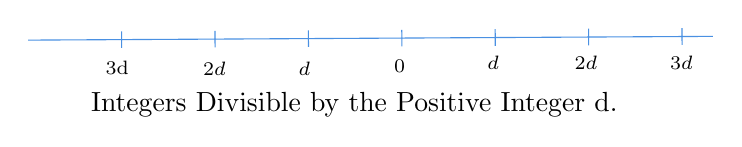
\begin{tikzpicture}[x=0.75pt,y=0.75pt,yscale=-1,xscale=1]
%uncomment if require: \path (0,300); %set diagram left start at 0, and has height of 300

%Straight Lines [id:da3876443293184153] 
\draw [color={rgb, 255:red, 74; green, 144; blue, 226 }  ,draw opacity=1 ]   (100,105) -- (211.82,104.39) -- (263.84,104.1) -- (429.82,103.19) (144.98,100.75) -- (145.02,108.75)(189.98,100.51) -- (190.02,108.51)(234.98,100.26) -- (235.02,108.26)(279.98,100.01) -- (280.02,108.01)(324.97,99.76) -- (325.02,107.76)(369.97,99.52) -- (370.02,107.52)(414.97,99.27) -- (415.02,107.27) ;

% Text Node
\draw (183,114.4) node [anchor=north west][inner sep=0.75pt]  [font=\scriptsize]  {$2d$};
% Text Node
\draw (136,114) node [anchor=north west][inner sep=0.75pt]  [font=\scriptsize] [align=left] {3d};
% Text Node
\draw (229,114.4) node [anchor=north west][inner sep=0.75pt]  [font=\scriptsize]  {$d$};
% Text Node
\draw (275,113.4) node [anchor=north west][inner sep=0.75pt]  [font=\scriptsize]  {$0$};
% Text Node
\draw (320,111.4) node [anchor=north west][inner sep=0.75pt]  [font=\scriptsize]  {$d$};
% Text Node
\draw (362,111.4) node [anchor=north west][inner sep=0.75pt]  [font=\scriptsize]  {$2d$};
% Text Node
\draw (408,111.4) node [anchor=north west][inner sep=0.75pt]  [font=\scriptsize]  {$3d$};
% Text Node
\draw (129,129) node [anchor=north west][inner sep=0.75pt]   [align=left] {Integers Divisible by the Positive Integer d.};


\end{tikzpicture}

\end{center}
\end{proof}
\begin{theorem}{Division Algorithm}
    Let a and d be integers with d $\textgreater$0. Then there are
unique integers q, r such that\begin{equation*}
    a = dq+r
\end{equation*}
with $0\leq r \textless d$.We refers to a,d,q,r as dividend divisor,quotient and remainder,respectively.
\end{theorem}

\section{Well ordering principle}

\begin{definition}
    The pair (A,($\leq$) is called a partially ordered set,or simply a poset,if $\leq$is a partial order on A
\end{definition}

\begin{definition}
    The pair (A, $\leq$) is called a totally
ordered set, or simply a chain, if $\leq$is a total
order on A.
\end{definition}

\begin{definition}
    Let (A, $\leq$) be a poset and B$\subseteq$A. Then
    \begin{enumerate}
        \item l $\in$ B is called the minimum in B if l $\leq$ b for all b $\in$ B.
        \item g $\in$ B is called the maximum in B if b $\leq$ g for all b $\in$  B.
    \end{enumerate}
\end{definition}



\begin{definition}
     Let (A, $\leq$) be a poset and B$\subseteq$A. Then
     \begin{enumerate}
         \item n $\in$ B is minimal in B $\Leftrightarrow$ $\lnot$($\exists$ b $\in$ B, b $\textless$ n).
         \item m $\in$ B is maximal in B $\Leftrightarrow \lnot (\exists b \in B, b >\textgreater m)$.
     \end{enumerate}
\end{definition}


\begin{theorem}
    Let (A, $\leq$) be a poset and B$\subseteq$A. Then
n $\in$ B is minimal in B $\Leftrightarrow$ $\exists$b $\in$ B, b $\leq$ n $\to$ b=n.
\end{theorem}
\begin{theorem}
    Let (A, $\leq$) be a poset and B$\subseteq$A. Then
n $\in$  B is maximal in B $\Leftrightarrow$ $\forall$b $\in$ B, m $\leq$ b $\to$ b=m.
\end{theorem}

\begin{definition}
    A totally ordered set (A, $\leq$) is
called a well ordered set if every nonempty
subset of A has a least element.
\end{definition}

\begin{theorem}{Well ordering principle}
    Every nonempty subset of N has a least element.
\end{theorem}
\begin{note}
    The set of natural numbers is well ordered.
\end{note}

\begin{theorem}{principle of Mathematical Induction}
Let S be a subset of natural numbers such that
\begin{enumerate}
    \item 0$\in$S;
    \item n$\in$S$\Rightarrow$n+1$\in$S
    
\end{enumerate}
    then S = N;
\end{theorem}
\begin{remark}
    Why Mathematical Induction is Valid?
    \footnote{Discrete mathematics and its applications}Why is mathematical induction a valid proof technique? The reason comes from $\textbf{the well- ordering property}$, listed in Appendix 1, as an axiom for the set of positive integers, which states that every nonempty subset of the set of positive integers has a least element. So, suppose we know that P (1) is true and that the proposition P (k) $\to$P (k + 1) is true for all positive integers k. To show that P(n) must be true for all positive integers n, assume that there is at least one positive integer for which P (n) is false. Then the set S of positive integers for which P (n) is false is nonempty. Thus, by the well-ordering property, S has a least element, which will be denoted by m. We know that m cannot be 1, because P (1) is true. Because m is positive and greater than 1, m - 1 is a positive integer. Furthermore, because m − 1 is less than m, it is not in S, so P (m - 1) must be true. Because the conditional statement P (m - 1) $\to$ P (m) is also true, it must be the case that P (m) is true. This contradicts the choice of m. Hence, P (n) must be true for every positive integer n.
\end{remark}

\begin{theorem}{Strong Induction}
    To prove that P (n) is true for all positive integers n, where P (n) is a propositional function, we complete two steps:
    \begin{enumerate}
        \item We verify that the proposition P (1) is true.
        \item We show that the conditional statement $[ P ( 1)  \land  P ( 2) \land  \cdotp  \cdotp  \cdotp  \land P ( k)]  \rightarrow  P ( k + 1)  $is true for all positive integers k.
    \end{enumerate}
\end{theorem}
\begin{note}
    Strong induction is sometimes called \textbf{the second principle of mathematical induction} or \textbf{complete induction}. 
\end{note}
\section{Modular arithmetic}
\begin{definition}
    Let a, n $\in$ Z with n  $\textgreater$ 0. We denote
by a mod n the remainder when a is divided by n.
\end{definition}

\begin{definition}
    Let a, b, n$\in$ Z with n $\textgreater$ 0. We say
that a is congruent to b modulo n, which is denote by a$\equiv$b (mod n), if $n | (a-b)$.
\end{definition}

\begin{theorem}
    Let n be a positive integer. Then the
congruent modulo n relation is an equivalence
relation on Z.
\end{theorem}
\begin{proof}
    \begin{itemize}
        \item reflexive:
        \item  transitive:
        \item symmetric:
    \end{itemize}
\end{proof}

\begin{definition}
    Let n be a positive integer. Then the quotient set
    \begin{equation*}
        Z_n=\{\overline{0},\overline{1},\cdots,\overline{n-1}\}=Z/R_n
    \end{equation*}
    is called the set of residue classes of integers modulo n,
where $R_n$ is the congruent modulo n relation.
\end{definition}
\begin{theorem}
    Let a, b, c, d, n $\in$ Z with n $\textless$ 0. Then
    \begin{enumerate}
        \item $a \equiv  b ( mod n)  \land  c \equiv  d ( mod n) \Rightarrow a + c \equiv  b + d ( mod n) .$
        \item $a \equiv  b ( mod n)  \land  c \equiv  d ( mod n) \Rightarrow a \cdotp  c \equiv  b \cdot  d ( mod n) .$
    \end{enumerate}
\end{theorem}

\section{Groups}
\subsection{Binary operations}
\begin{definition}
    A binary operation on a nonempty set A is a mapping 
$\odot$: A$\times$A $\to$A.

A binary operation $\odot$  on A is associative if a(bc) =( ab) c for all a,b,c$\in$ A.
A binary operation $\odot$  on A is commutative if ab=ba for all a,b$\in$ A.

\end{definition}

\begin{definition}
    Let $\odot$ : A$\times$ A $\rightarrow$  A be a binary operation on A. Then
\begin{enumerate}
\item An element l$\in$ A is called a left identity if la=a for all a$\in$ A. 
\item An element r$\in$ A is called a right identity if ar=a for all a$\in$ A.
\item An element e$\in$ A is called an identity if ae=ea=a for all a$\in$ A.
\item An element a$\in$ A is called an idempoten if $a^2=a$,$\exists a\in$A.
\end{enumerate}
\end{definition}

\begin{theorem}
    Let $\odot$ : A$\times$ A $\rightarrow$ A be a binary operation on A. If l and r are respectively left and right identities in A, then l=r is an identity
\end{theorem}


\begin{theorem}
    Let $\odot$ : A$\times$ A $\rightarrow$ A be a binary operation on A. Then the identity in A is unique if it exists.
\end{theorem}

\subsection{Semigroups}
\begin{definition}[Groupoid(群胚)]
A groupoid ( G,$\odot$ )  is a nonempty settogether with a binary operation $\odot$  on G.
\end{definition}

\begin{definition}[Semigroups(半群)]
    A groupoid ( G,$\odot$ ) is called a semigroup if the operation $\odot$  is associative.
\end{definition}

\begin{definition}[monoid(幺半群)]
    A semigroup ( G,$\odot$ )  is called a monoid if it contains an identity.
\end{definition}
\begin{remark}
    Group has only one idempotent.But probality has not one idempotent.
    \begin{example}
        A = [0,1],$a\lor b$ = max$\{a,b\}$,$S^{'}= (A,\lor)$,we can know\begin{equation*}
            \forall a \in A \quad a\lor a = a \Rightarrow aRa = a 
        \end{equation*}
        The idempotent has more than one in semigroup.
    \end{example}
\end{remark}

\begin{definition}[Abelian(阿贝尔群)]
    A semigroup ( G,$\odot$ ) is said to be Abelian if the operation $\odot$  is commutative.
\end{definition}


\subsection{Groups}
\begin{definition}
    A monoid ( G,$\odot$ ) with identity e is a called a group if for every a in G, there exists b in Gsuch that ab=ba=e. The element b, denoted by b=$a^{-1}$, is called the inverse of a.
\end{definition}

\begin{definition}
    The order of a group ( G,$\odot$  ) is the cardinality of the set G.
\end{definition}

\begin{example}
    \begin{enumerate}
        \item groups($\mathbb{Z}$,+),The identity is 0.Inverse is -a.
        \item groups($\mathbb{Q}^*$,$\cdot$),The identity is 1.Inverse is 1/a.
        \item GL(n,R)=$R^{n\times n}$={A$|$is an n$\times$n real matrix} is a groups under the multipliaction
    \end{enumerate}
\end{example}

\begin{proposition}
    \begin{enumerate}
        \item The identity e is unique.
        \item The inverse $a^{-1}$ is unique for each a in G.
        \item The inverse of $a^{-1}$ is the element a.
        \item The inverse of ab is the element $b^{-1}$$a^{-1}$.
        \item The identity e is the unique idempotent element in G
        \item For all a,b,c$\in$G, ab=ac $\Rightarrow$ b=c
        \item For all a,b,c$\in$G, ba=ca $\Rightarrow$ b=c
        \item For a,b$\in$G, the equations ax=b and ya=b have unique solutions x=$a^{-1}$b and y=b$a^{-1}$, respectively.
    \end{enumerate}
\end{proposition}

\begin{proof}

\begin{enumerate}
    \item Assume that $e_1$ and $e_2$ are both identities.so
    \begin{equation*}
        e_1=e_1*e_2=e_2
    \end{equation*}
    the identity is unique.
    \item Assume that $a_1^{-1},a_2^{-1}$ are both inverses.we know
    \begin{equation*}
        a_1^{-1}*(e)=a_1^{-1}*(a*a_2^{-1})=e*a_2^{-1}=a_2^{-1}
    \end{equation*}
    \item According definition, We can know $a^{-1}$ is inverse of a
    \item Note first $ab*(b^{-1}a^{-1})=e$,so The inverse of ab is the element $b^{-1}$$a^{-1}$
    \item Note first that e is  idempotent.If$a^2=a$,the we can deduce that e=$a^{-1}a=a^{-1}a^2=ea=a$
    \item If ab=ac,then we have \begin{equation*}
        b=eb=(a^{-1}a)b=a^{-1}ac=c
    \end{equation*}
    \item etc
    \item if ax=b and ya=b we have \begin{equation*}
        x=ex=(a^{-1}a)x=a^{-1}ax=a^{-1}b
    \end{equation*}
 \end{enumerate}
    
\end{proof}



\begin{theorem}
    

    A semigroup ( G,$\odot$ )  is a group if and only if it satisfies the following:
    \begin{enumerate}
        \item G has a left identity l;
        \item  for all a $\in$ G, $\exists$ $a^{*}$$ \in$ G such that $a^{*}$ a=l
    \end{enumerate}
\end{theorem}

\begin{proof}
    $\Rightarrow$ Obviously that is true\\
    $\Leftarrow$ Assume that G is (G,Q) is a semigroup such that ax=b and ya=b.Given $b_0\in G$,the equation $yb_0=b_0$ is a solution y=l.For every a$\in$G.the equation $b_0x=a$ as a solutionx=$C_0$It fllows that la=l($b_0c_0)=b_0c_0=a$,Which shows that l is note also that the equation ya=l has a solution y=$a^*$ the left inverse of a.Therefor G is a group.
\end{proof}
Similarly we can conclude that:
\begin{theorem}
    A semigroup ( G,$\odot$ ) is a group if and only if it satisfies the following:
    \begin{enumerate}
        \item G has a right identity r
        \item for all a $\in$ G, $\exists$ $a^{*}$ $\in$ G such that aa*=r.
    \end{enumerate}
\end{theorem}

\begin{theorem}
     A semigroup ( G,$\odot$ )  is a group if and only if for all a,b $\in$ G, the equations ax=b and ya=b have solutions in G
\end{theorem}
\begin{proof}
    $\Rightarrow$ Straightforward\\
    $\Leftarrow$ Assume that G is semigroup such that ax=b and ya=b have solutions.Given $b_0\in G$,the equation $yb_0=b_0$ has a solution y = l.For every a$\in$G,the equation $b_0x=a$ has a solution $x=c_0$ It follows that la=l($b_0c_0)=b_0c_0=a$ which shows that l is a left identity.Note that the equation ya=l has a solution y=$a^*$.Hence,$a^*$is the left inverse of a.
    According Theorem2.29 we know that it is a group.
\end{proof}
\newpage

\begin{introduction}[Keywords]
    \item subgroup 子群
    \item trivial subgroup 平凡子群
    \item  subgroup generated by X 由X生成的子群
    \item cyclic 循环的
    \item generator 生成元
    \item finitely generated 有限生成的
\end{introduction}
\subsection{Subgroup}

\begin{definition}
A nonempty set H of a group ( G,$\odot$ )  is called a subgroup of G, denoted by H $\leq$ G, if H forms a group under the binary operation $\odot$  of G( restricted to its subset H) . 
\end{definition}


\begin{theorem}
    

    A nonempty set H of a group ( G,$\odot$ ) is called a subgroup of G, denoted by H  G, if it satisfies the following conditions:
    \begin{enumerate}
        \item H contains the identity of G;
        \item For all x,y$\in$ H, xy$\in$ H; $\left( i.e., H^{2}\subseteq H \right)$
        \item For all x,y$\in$ H, $xy^{-1}$$ \in $H. $\left( i.e., H^{-1}  \subseteq H\right)$
    \end{enumerate}
\end{theorem}
\begin{definition}
    A nonempty set H of a group(G,$\circ$) is called a subgroup of G,if it satisfied
    \begin{enumerate}
        \item $\forall x,y\in H$,xy$\in$h
        \item H contains the identity of G
        \item $\forall$ y$\in H,y^{-1}\in H$
    \end{enumerate}
\end{definition}
\begin{note}
    \begin{enumerate}
        \item 1,2 can proves the G is submoinod.
        \item 1,2,3 can proves the G is subgroup
    \end{enumerate}
\end{note}

\begin{theorem}
    H is a sub group of G
    \begin{enumerate}
        \item H$\leq$G
        \item $\forall x,y\in H$,$xy\in H$ and $y^{-1}\in H$
        \item $\forall$ x,y$\in H$,$xy^{-1}\in H$
    \end{enumerate}
\end{theorem}

\begin{proof}
    3$\Rightarrow$1
    Assum that $xy^{-1}\in H$ whenever x,y$\in$H,since $H\neq \emptyset$,there exits some a $\in$ H.Thus e = $aa^{-1}\in H$,Hence 
    \begin{equation*}
        b^{-1}=eb^{-1}\in H
    \end{equation*}
    \begin{equation*}
        ab = a(b^{-1})^{-1}\in H
    \end{equation*}
    Therefore,H$\leq$G
\end{proof}

\newpage

\begin{theorem}
    If G is a group and $\underset{i\in I}{\cap}H_i$,then $\cap_{i\in I}H_i$is a subgroup of G.
\end{theorem}

\begin{proof}
    Let H = $\underset{i\in I}{\cap}H_i$,if x,y$\in$H,then x,y$\in H_i$,for all $i\in I$.\\Thus $xy^{-1}\in H_i \leq G$for all i$\in$I.Hence $xy^{-1}\in H$.Therefore H$\leq$G
\end{proof}

\begin{note}
    The intersection of some subgroups of a group G is also a subgroup of G.
\end{note}

\begin{definition}
    Let G be a group and x$\subseteq$G.Then\begin{equation*}
        <x>=\cap \{H|X\subseteq H \leq G\}
    \end{equation*}
    is called \textbf{the subgroup of G generated by X}
\end{definition}
\begin{note}
    The subgroup generated by the set X is the smallest subgroup of G containing X.
\end{note}
\begin{note}
    <$\emptyset$>={e}
\end{note}
\begin{note}
    G中的真子群分布是不均匀的,不是一直都是一层包含一层的关系,很大可能是离散的每个群包含的元素有的相同,有的不同,比如$Z_6$中的剩余类群就是不一样的(2,4)和(0,3)。
\end{note}

\begin{definition}
    Let G be a group and H = <X>$\leq$ G,Then
    \begin{enumerate}
        \item The elements of X are called the generated of H.
        \item H is said to be finitely generated if it has a finite set of generators.
        \item H is said to be cyclic if it can be generated by a single generator.
    \end{enumerate}
\end{definition}


\begin{theorem}
    Let G be a group and $\emptyset \neq X \subseteq G$. If H is the set of all finite product of elements in X $\cup X^{-1}$,then H is the subgroup of generated by X.
\end{theorem}
\begin{note}
    The subgroup generated by X contains exactly all the finite product elements in X or$ X^{-1}$
\end{note}

\begin{theorem}
    Let G be a group and $\emptyset \neq X\subseteq G$.Then
    \begin{equation*}
        <X>=\{a_1^{k_1}a_2^{k_2}\cdots a_n^{k_n}\}
    \end{equation*}
    \begin{enumerate}
        \item $a^0=e,a^2=aa,a^{-2}=(a^2)^{-1}$
        \item <X> contains excutly all the finite product of elements in X or $X^{-1}$
    \end{enumerate}
\end{theorem}
\newpage
\begin{introduction}[Keywords]
    \item homomorphism 同态
    \item  homomorphic image 同态像
\item  monomorphism 单同态
\item  epimorphism 满同态
\item  endomorphism 自同态
\item automorphism 自同构
\item isomorphism 同构
\item  isomorphic to 同构于
\item  kernel 核
\end{introduction}
\subsection{Homomorphisms}
\begin{definition}
    Let(F,$\odot$) and (K,+) be semigroups.
    A mapping f:G$\to$K is called a homomorphism if \begin{equation*}
        f(a\odot b)=f(a)+f(b)
    \end{equation*}
    for all a,b$\in$ G.
\end{definition}
\begin{remark}
    A homomorphism between two semigroups is a mapping which is compatible to the binary operation defined on the semigroups
\end{remark}

\begin{definition}
    Let f:G$\to$H be a homomorphism.Then f is called
    \begin{enumerate}
        \item a monomorphism if it is injective
        \item an epimorphism if it is surjective
        \item an isomorphism if it is bijective
        \item an endomorphism if G=H
        \item an automorphism if G=H and f is bijective
    \end{enumerate}
\end{definition}
\begin{definition}
    Let G and H be semigroups.Then G is said to be isomorphic to H if there exists an isomorphism from G to H.This is denoted by G $\cong$ H
\end{definition}
\begin{note}
    The realtion $\cong$ is an equivalence relation
\end{note}
\begin{definition}
   Let f: G$\to$K be a homomorphism of groups Then Im(f)=f(G) is called the homomorphic image of G,and ker(f) =$f^{-1}(<e_K>)$ is called the kernel of f 

    \begin{enumerate}
        \item Ker(f) = $f^{-1}(\{e_K\})$=$\{a\in G|f(a)=e_K\}$
        \item Ker(f)是$E_k$原象集
        \item $e_G \in Ker(f)$
    \end{enumerate}
\end{definition}
\begin{proof}
    1$\Rightarrow$3,First assume that f is monomorphism,since $f(e_G)=e_K$,we have $e_G\in Ker(f)=f^{-1}(\{e_K\})$,Let $a\in Ker(f)$,Then f(a)=$e_K=f(e_G)$.since f is injective it follows that a = $e_G$ ,Therefore Ker(f)=\{$e_G$\}\\
    3$\Rightarrow$1 Let a,b belongs to G,f(a)=f(b).Then \begin{equation*}
        f(ab^{-1})=f(a)f(b^{-1})=f(a)f(a^{-1})=e_K
    \end{equation*}
    Thus $ab^{-1}\in Ker(f)=\{e_G\}$,That is $ab^{-1}=e_G$,Hence $a=(b^{-1})^{-1}=b$,Therefore f is a monomorphism
\end{proof}
\begin{remark}
    Let G be an Abelian group consider the mapping f:G$\to$ G given by \begin{equation*}
        f(x)=X^{-1}
    \end{equation*}
    Show that f is an automorphism of groups
\end{remark}

\begin{definition}
    Let f:G$\to$K be a homoorphism of groups.Then Im(f)=f(G) is called the homomorphic image of G,and Ker(f)=$f^{-1}(\{e_k\}$ is called the kernel of f
\end{definition}

\begin{example}
    Let $3Z=\{3n|n\in Z\}$ . It can be seenthat 3Z is a subgroup of the additive group ofintegers. Consider the mapping f: Z$ \rightarrow $ 3Z given by f(n) =3n. One can verify that f is anisomorphism of groups. 
\end{example}

\begin{proposition}
    Let A,B,C be subgroups.Let f:A$to$B and g:B$\to$C be mappings.Then we have:
    
\begin{enumerate}
 
\item If f and g are homomorphisms, then g$\circ$ f is a homomorphism.
\item  If f and g are monomorphisms, then g$\circ$ f is a monomorphism.
\item  If f and g are epimorphisms, then g$\circ$ f is an epimorphism.
\item  If f and g are isomorphisms, then g$\circ$ f is an isomorphism.

\end{enumerate}
\end{proposition}
\begin{proposition}
    Let $f$:G$\to$K be a homomorphism of groups.Then we have:
    \begin{enumerate}
        \item $f$($e_G$)=$e_k$.
        \item $f$($x^{-1}$)=$(f(x))^{-1}$.
    \end{enumerate}
\end{proposition}
\begin{proof}
\begin{enumerate}
    \item Since f is a group homomorphism,$f(e_G)f(e_G)=f(e_Ge_G)=f(e_G)$,The shows that $f(e_G)$ is idempotent.Note also that $e_K$ is the unique idenpotent in K,Thus $f(e_G)=e_K$
    \item     let $x\in G$,since
    \begin{equation*}
        f(x)\cdot f(x^{-1})=f(e_G)=e_k\Rightarrow f(x)=(f(x^{-1}))^{-1}
    \end{equation*}
\end{enumerate}
\end{proof}


–\begin{note}
    The identity and inverses are preserved under the homomorphism of groups
\end{note}


\begin{proposition}
    Let f:G$\to$K be a homomorphism of groups.Then we have:
    \begin{enumerate}
        \item $K_1\leq K \Rightarrow f^{-1}(K_1)\leq G.$
        \item $G_1\leq G \Rightarrow f(G_1)\leq K.$
    \end{enumerate}
\end{proposition}

\begin{proof}
    \begin{enumerate}
        \item Note first that $f^{-1}(K_1) \neq \emptyset$,since $f(e_G)=e_K\in K_1\leq K$.Let$x,y\in f^{-1}(K_1)$ Then f(x),f(y)$\in K_1$,since$K_1 \leq K$,it follows that $f(x)(f(y))^{-1}=f(x)f(y^{-1})=f(xy^{1})\in K_1$,Thus $xy^{-1}\in f^{-1}(K_1)$,Which shows that $f^{-1}\leq G$ 
        \item Note first that $f(G_1\neq \emptyset$ since $e_K = f(e_G)\in f(G_1)$,If $x,y\in G_1 \leq G$and $f(x_1y_1^{-1})=f(x_1)f(y_1^{-1})=f(x_1)f(y_1)^{-1}=xy^{-1}\in f(G_1$.Hence $f(G_1)\leq K$
    \end{enumerate}
\end{proof}

% $\forall x\in A,y\in B$,f(x)=y:
% \begin{center}
    

% \tikzset{every picture/.style={line width=0.75pt}} %set default line width to 0.75pt        

% \begin{tikzpicture}[x=0.75pt,y=0.75pt,yscale=-1,xscale=1]
% %uncomment if require: \path (0,300); %set diagram left start at 0, and has height of 300

% %Shape: Ellipse [id:dp4792424517897742] 
% \draw  [fill={rgb, 255:red, 74; green, 144; blue, 226 }  ,fill opacity=1 ] (100,88.14) .. controls (100,55.64) and (115.67,29.29) .. (135,29.29) .. controls (154.33,29.29) and (170,55.64) .. (170,88.14) .. controls (170,120.65) and (154.33,147) .. (135,147) .. controls (115.67,147) and (100,120.65) .. (100,88.14) -- cycle ;
% %Shape: Ellipse [id:dp6158808052780425] 
% \draw  [fill={rgb, 255:red, 74; green, 144; blue, 226 }  ,fill opacity=1 ] (352,88.14) .. controls (352,55.64) and (367.67,29.29) .. (387,29.29) .. controls (406.33,29.29) and (422,55.64) .. (422,88.14) .. controls (422,120.65) and (406.33,147) .. (387,147) .. controls (367.67,147) and (352,120.65) .. (352,88.14) -- cycle ;
% %Curve Lines [id:da5524865968284174] 
% \draw    (130.82,80.29) .. controls (157.69,48.45) and (318.21,25.52) .. (382.86,73.56) ;
% \draw [shift={(383.82,74.29)}, rotate = 217.44] [color={rgb, 255:red, 0; green, 0; blue, 0 }  ][line width=0.75]    (10.93,-3.29) .. controls (6.95,-1.4) and (3.31,-0.3) .. (0,0) .. controls (3.31,0.3) and (6.95,1.4) .. (10.93,3.29)   ;

% % Text Node
% \draw (128,147) node [anchor=north west][inner sep=0.75pt]   [align=left] {A};
% % Text Node
% \draw (382,147) node [anchor=north west][inner sep=0.75pt]   [align=left] {B};
% % Text Node
% \draw (122,143.4) node [anchor=north west][inner sep=0.75pt]    {$$};
% % Text Node
% \draw (258,30) node [anchor=north west][inner sep=0.75pt]   [align=left] {{\fontfamily{helvet}\selectfont f}};


% \end{tikzpicture}

% \end{center}

% $,\exists x\in A_1,B_1\in B_1$

\subsection{Cyclic groups}
\begin{definition}
    Let G be a group and $X\subseteq G$.Then
    \begin{equation*}
        <X> = \cap \{H|X\subseteq \leq G\}
    \end{equation*}
    is called the \textbf{subgroup of G generated by X}
\end{definition}


\begin{definition}
    Let G be a group and $H\leq G$.Then H is said to be cyclic if $H =<a>$ for some a in H
\end{definition}

\begin{definition}
    Let G be a group and a$in$G.The orderof the element a,denoted by $|a|$,is the order of the cyclic groups generated by a
\end{definition}

\begin{definition}[cyclic groups]
    Let n be a positive integer.Then the quotient set \begin{equation*}
        \mathzz{Z}_n = {\overline{0},\overline{1},\cdots,\overline{n-1}}
    \end{equation*}
\end{definition}
\begin{example}
we can know the equation that $\overline{r}=\{k\in Z|r\equiv k(mod n)\}=\{k\in Z\ | \k\  mod\ n = r\}$
\\
    The set $\mathzz{Z}$ forms a groups under the binary operration:
    \begin{equation*}
        \overline{r} + \overline{s}=\overline{r+s}
    \end{equation*}
\end{example}


\begin{example}
\begin{enumerate}
    \item     The additive groups of integers is an  infinite cyclic group generated by the genrator 1.
    \item The groups $\mathh{Z}_n$ consisting of all the residue classes of integer modulo n is a finite cyclic group generated by the generator  $\overline{1}$
\end{enumerate}
\end{example}
\begin{example}
    Consider the residue class groups $Z_6$.As shown in the foregoing,\{$\overline{0},\overline{3}$\} and $\{\overline{0},\overline{2},\overline{4}\}$are subgroups of $Z_6$.In addition,it is easy to verify the following facts:
\begin{equation*}
|\overline{3}|=|<\overline{3}>|=|\{|\overline{3},\overline{0}\}|=2
\end{equation*}

\begin{equation*}      
  |\overline{0}+\overline{2}+\overline{4}|=3
\end{equation*}
\end{example}


\end{document}
